\chapter{Analoge antialiasing og rekonstruktions filtre}\label{kap:analog_filter}

\begin{figure}[h]
	\vspace*{-1 cm}
	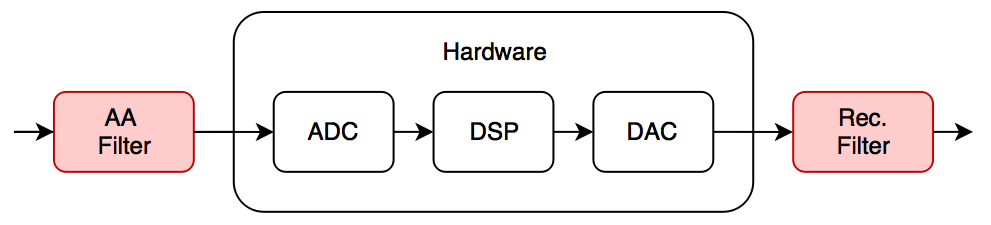
\includegraphics[width=8cm]{billeder/flow_filter}
	\vspace{0.5 cm}
\end{figure}

\emph{Kapitlet her, vil beskrive hvilke analoge filtre der skal anvendes for at være i stand til at modulere signalet efter designspecifikationerne. Dertil vil filtrene også blevet designet og simuleret i dette kapitel.}
